\section{Overview}\label{sec:overview}

\begin{figure}
  \centering
  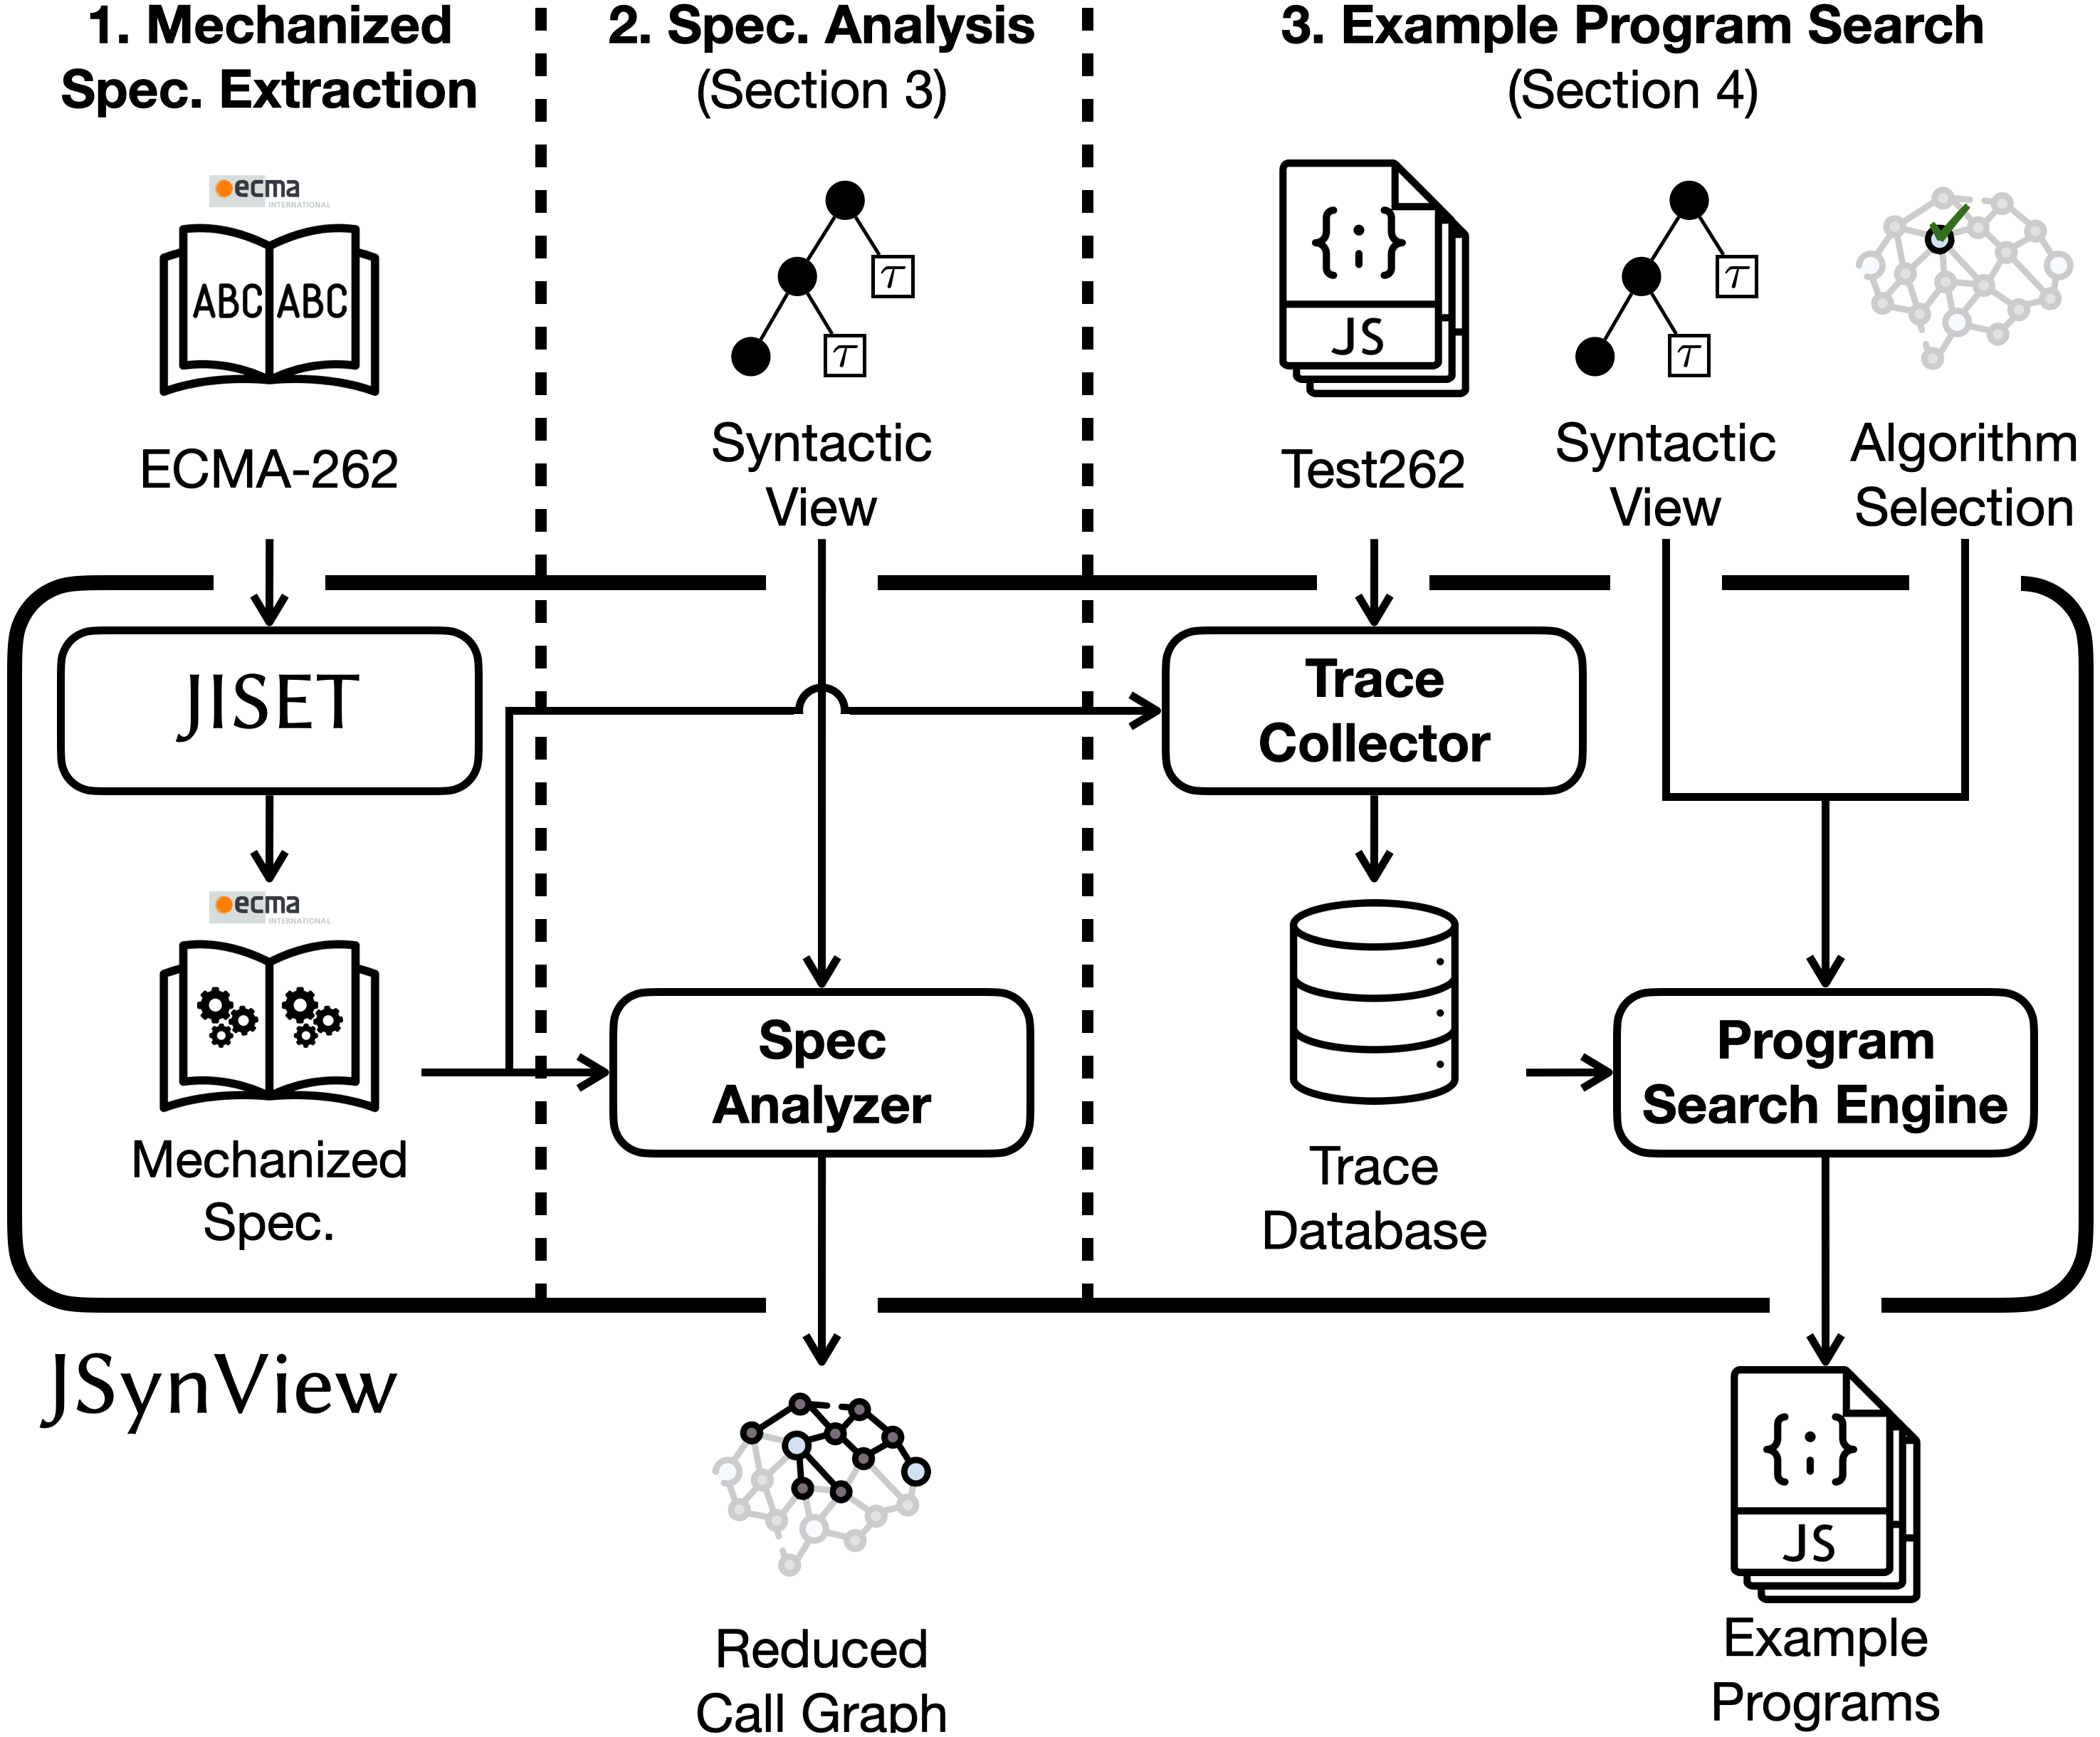
\includegraphics[width=\columnwidth]{img/overall.png}
  \caption{Overall structure of $\tool$}
  \label{fig:overall}.
\end{figure}

This section explains the overall structure of $\tool$ depicted in
Figure~\ref{fig:overall} with simple examples.  It consists of two main phases:
1) \textit{language specification reduction} and 2) \textit{example program
search}.


\subsection{Language Specification Reduction}\label{sec:reduce-spec}

% demonstrate the overall structure of $\tool$ depicted in
% Figure~\ref{fig:overall}.  It consists of three components:
% 1) specification extraction, 2) type analysis, and 3) bug detection.
% 
% % However, because the specification is written in
% % English, we should manually construct call graphs from the \esalg{Evaluation}
% % algorithm to check the reachability.  % As a result, the call graph consists of
% % \inred{107} algorithms, including the \esalg{Call} algorithm, which means that
% % the addition operator might cause implicit function calls.  
% 
% This section explains the motivation of this work.  We first shows how we can
% understand the detailed semantics by reducing the language specification with a
% given syntactic view.  Then, we show the effect of example programs found in the
% conformance test suite for each algorithm in the reduced specification.
% 
% 
% \begin{figure}
%   \centering
%   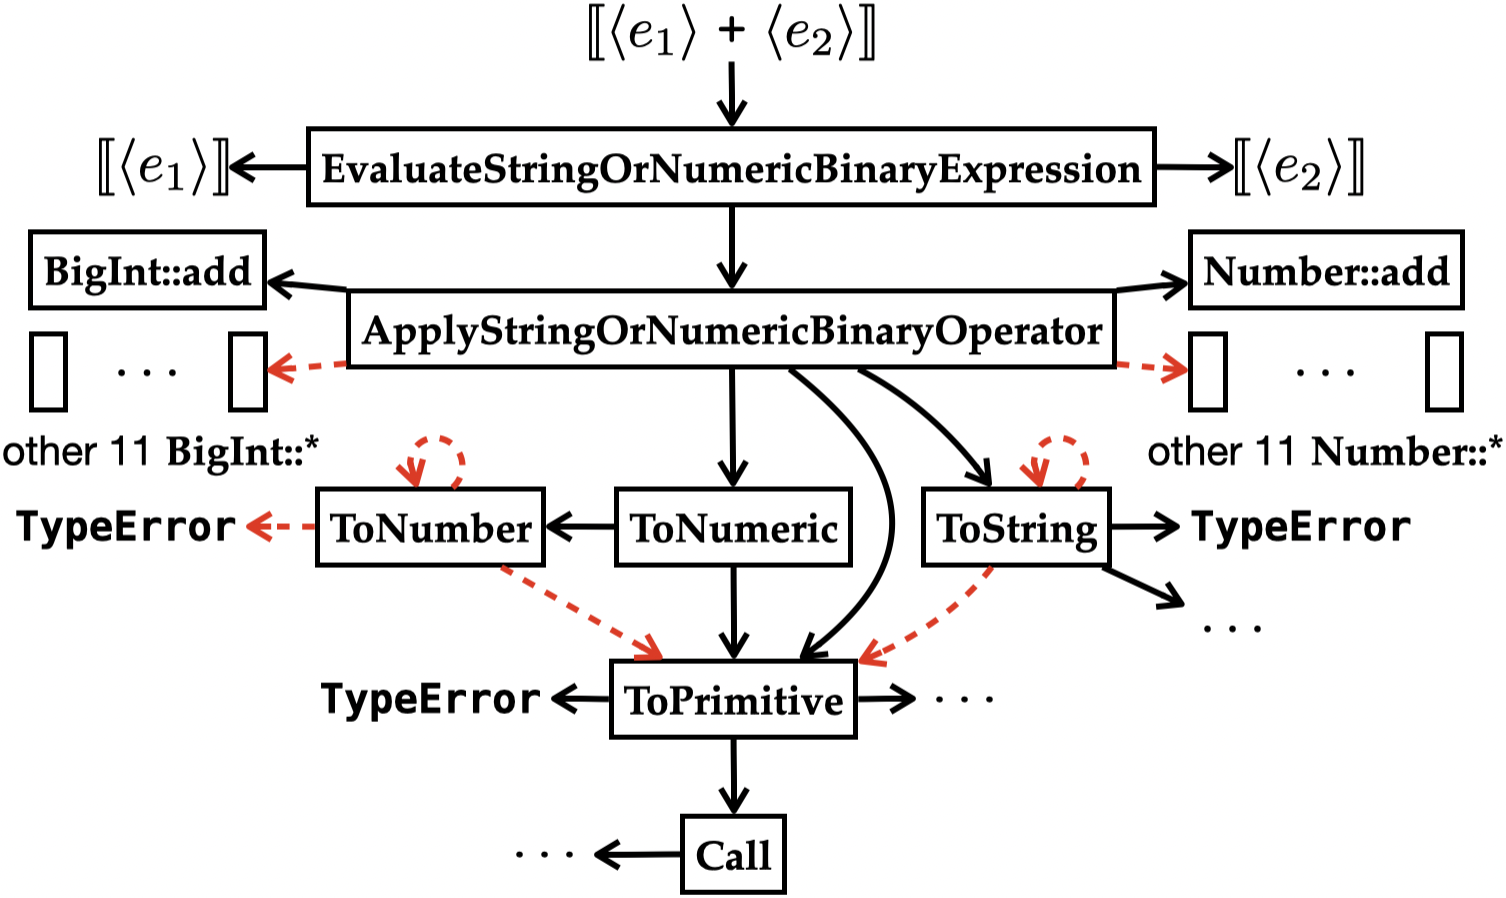
\includegraphics[width=\columnwidth]{img/add-basic.png}
%   \caption{A call graph of the JavaScript language specification reduced with a
%   syntactic view: $\svhole{\expr_1} \; \code{+} \; \svhole{\expr_2}$}
%   \label{fig:add-basic}.
% \end{figure}
% 
% Assume that we want to understand the detailed semantics of JavaScript addition
% operator (\code{+}) by referring to the latest ECMA-262 (ES12, 2021).  Then, we
% can utilize a syntactic view $\svhole{\expr_1} \; \code{+} \; \svhole{\expr_2}$
% where $\svhole{\expr_1}$ and $\svhole{\expr_2}$ denote arbitrary expressions.
% Then, $\tool$ first automatically find the \esalg{Evaluation} algorithm of the
% addition operator shown in Figure~\ref{fig:add-eval}.  In most cases, most
% abstract algorithms in ECMA-262 are not defined alone but utilizes other
% algorithms.  This algorithm also utilizes another algorithm named
% \esalg{EvaluateStringOrNumericBinaryExpression}.
% 
% Figure~\ref{fig:add-basic} depicts the call graph of the language specification
% starting from the \esalg{Evaluation} algorithm.  In this graph, a node denotes
% 1) an abstract algorithm (box), 2) evaluation of syntactic view ($\sem{-}$), or
% 3) an exception (bold without box), and an arrow denotes a call edge. Each
% reachable node represents possible behaviors of the addition operator.  For
% example, the \esalg{Call} algorithm is used to call the \eswrd{[[Call]]}
% internal method of a JavaScript function object.  It means that a JavaScript
% function might be invoked during the evaluation of the addition operator.  In
% addition, the addition operator might throw a \esval{TypeError} exception
% because it is reachable from the \esalg{Evaluation} algorithm through
% \esalg{ToNumber}, \esalg{ToString}, and \esalg{ToPrimitive}.
% 
% However, this call graph contains invalid edges for the evaluation of the
% addition operator.  Red dotted arrows in Figure~\ref{fig:add-basic} represents
% such cases.  For example, \esalg{ApplyStringOrNumericBinaryOperator} only
% invokes two different numeric methods \esalg{BigInt::add} and
% \esalg{Number::add} for the evaluation of the addition oeprator.  Other 22
% numeric methods, such as \esalg{BigInt::subtract} and \esalg{Number::divide},
% are unreachable.  Moreover, \esval{TypeError} is throwable only in
% \esalg{ToPrimitive} and \esalg{ToString} but not in \esalg{ToNumber} for the
% addition operator.
% 
% 
% \subsection{Advanced Syntactic Views}\label{sec:adv-syn-view}
% 
% Beyond syntactic restriction, we can give a more restriction to a syntactic view
% with types of evaluation results.  For example, assume that we want to
% understand the addition between string values, and a syntactic view
% $\svhole{\expr_1: \text{String}} \; \code{+} \; \svhole{\expr_2: \text{String}}$
% represents such cases.  Then, the following call graph is produced with this
% syntactic view:
% \begin{figure}[H]
%   \centering
%   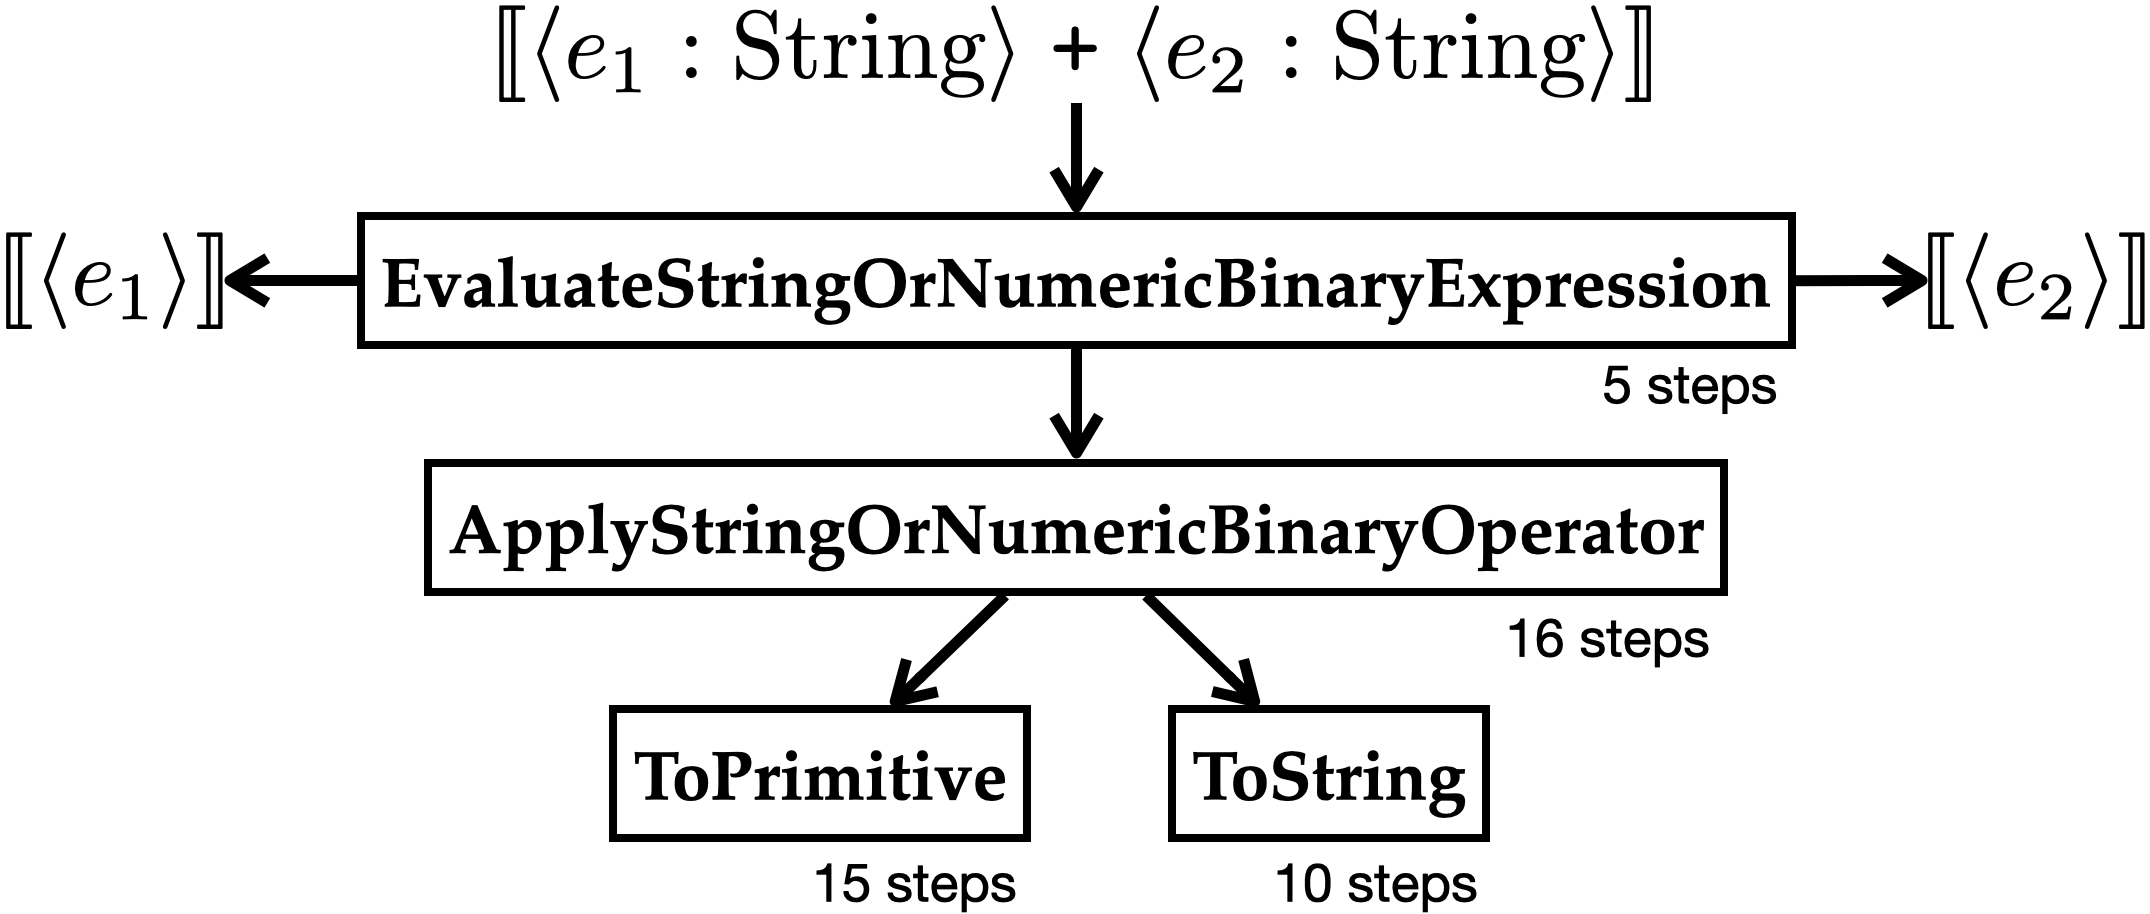
\includegraphics[width=.8\columnwidth]{img/add-str.png}
% \end{figure} \noindent
% Using this call graph, we can more understand behaviors of the addition
% oeprator.  First, the addition between string values do not throw any exceptions
% because there is no reachable exceptions in this call graph.  Besides, the
% string addition cannot invoke other JavaScript functions because the
% \esalg{Call} algorithm is no longer rechable from the \esalg{Evaluation}
% algorithm.
% 
% We can even define a syntactic view with exceptions $\svhole{\expr_1: \bot} \;
% \code{+} \; \svhole{\expr_2: \bot}$.  With this syntactic view, the call graph
% is changed as follows:
% \begin{figure}[H]
%   \centering
%   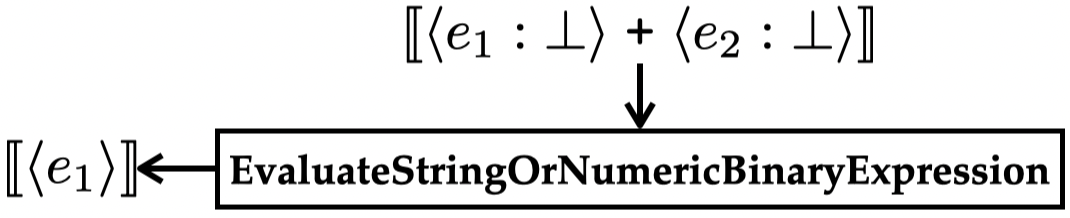
\includegraphics[width=.7\columnwidth]{img/add-exc.png}
% \end{figure} \noindent
% In this case, we notice that only left operand is evaluated when both left and
% right operand throw exceptions.
% 
% Moreover, we can combine different language features in syntactic views.  A
% syntactic view
% $\svhole{\expr_1: \text{Number}} \;
% \code{+} \;
% \svhole{\expr_2: \text{Number}} \;
% \code{*} \;
% \svhole{\expr_3: \text{Number}}$
% represents the combination of numeric addition and multiplication, and it
% produces the following call graph:
% \begin{figure}[H]
%   \centering
%   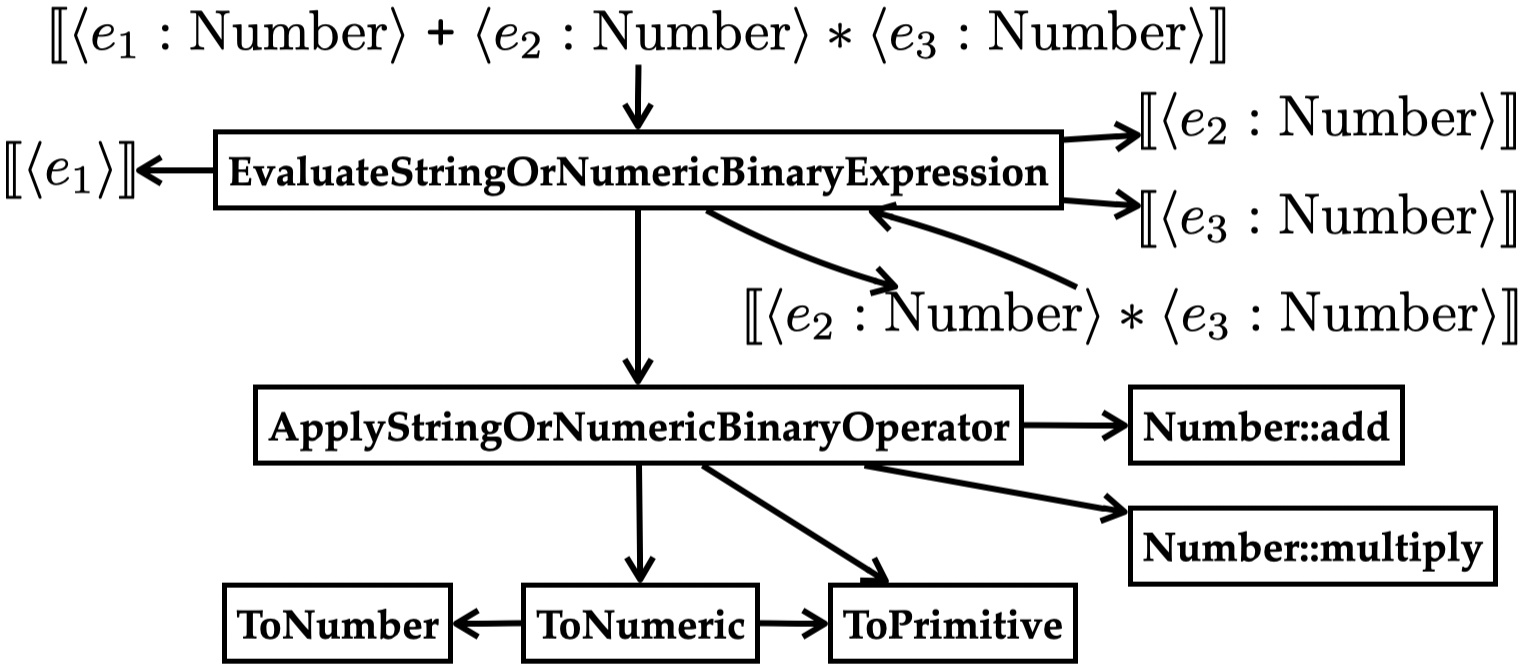
\includegraphics[width=\columnwidth]{img/add-mul.png}
% \end{figure}
% 
% 
% 
% \subsection{Finding Example Programs}\label{sec:find-prog}
% 
% \begin{itemize}
%   \item In Figure~\ref{fig:add-basic}
%     \begin{itemize}
%       \item TypeError in ToString:
%         \code{test/language/expressions/addition/symbol-to-string.js}
%       \item Call:
%         \code{test/language/expressions/addition/S11.6.1\_A2.2\_T1.js}
%     \end{itemize}
% \end{itemize}
